\documentclass[11pt,a4paper]{report}
\usepackage{marvosym}

\assignment{2}
\group{...}
\students{..........}{..........}

\begin{document}

\maketitle

Answer to the questions by adding text in the boxes. You may answer in either \textbf{French or English}. Do not modify anything else in the template.  The size of the boxes indicate the place you \textbf{can} use, but you \textbf{need not} use all of it (it is not an indication of any expected length of answer). \textbf{Be as concise as possible! A good short answer is better than a lot of nonsense!}
%\bigskip

\section{Exercises (5~pts)}

\textit{The following figure assigns a unique letter to each node, and a unique number to each branch. Use it to answer the following questions.}
\begin{center}
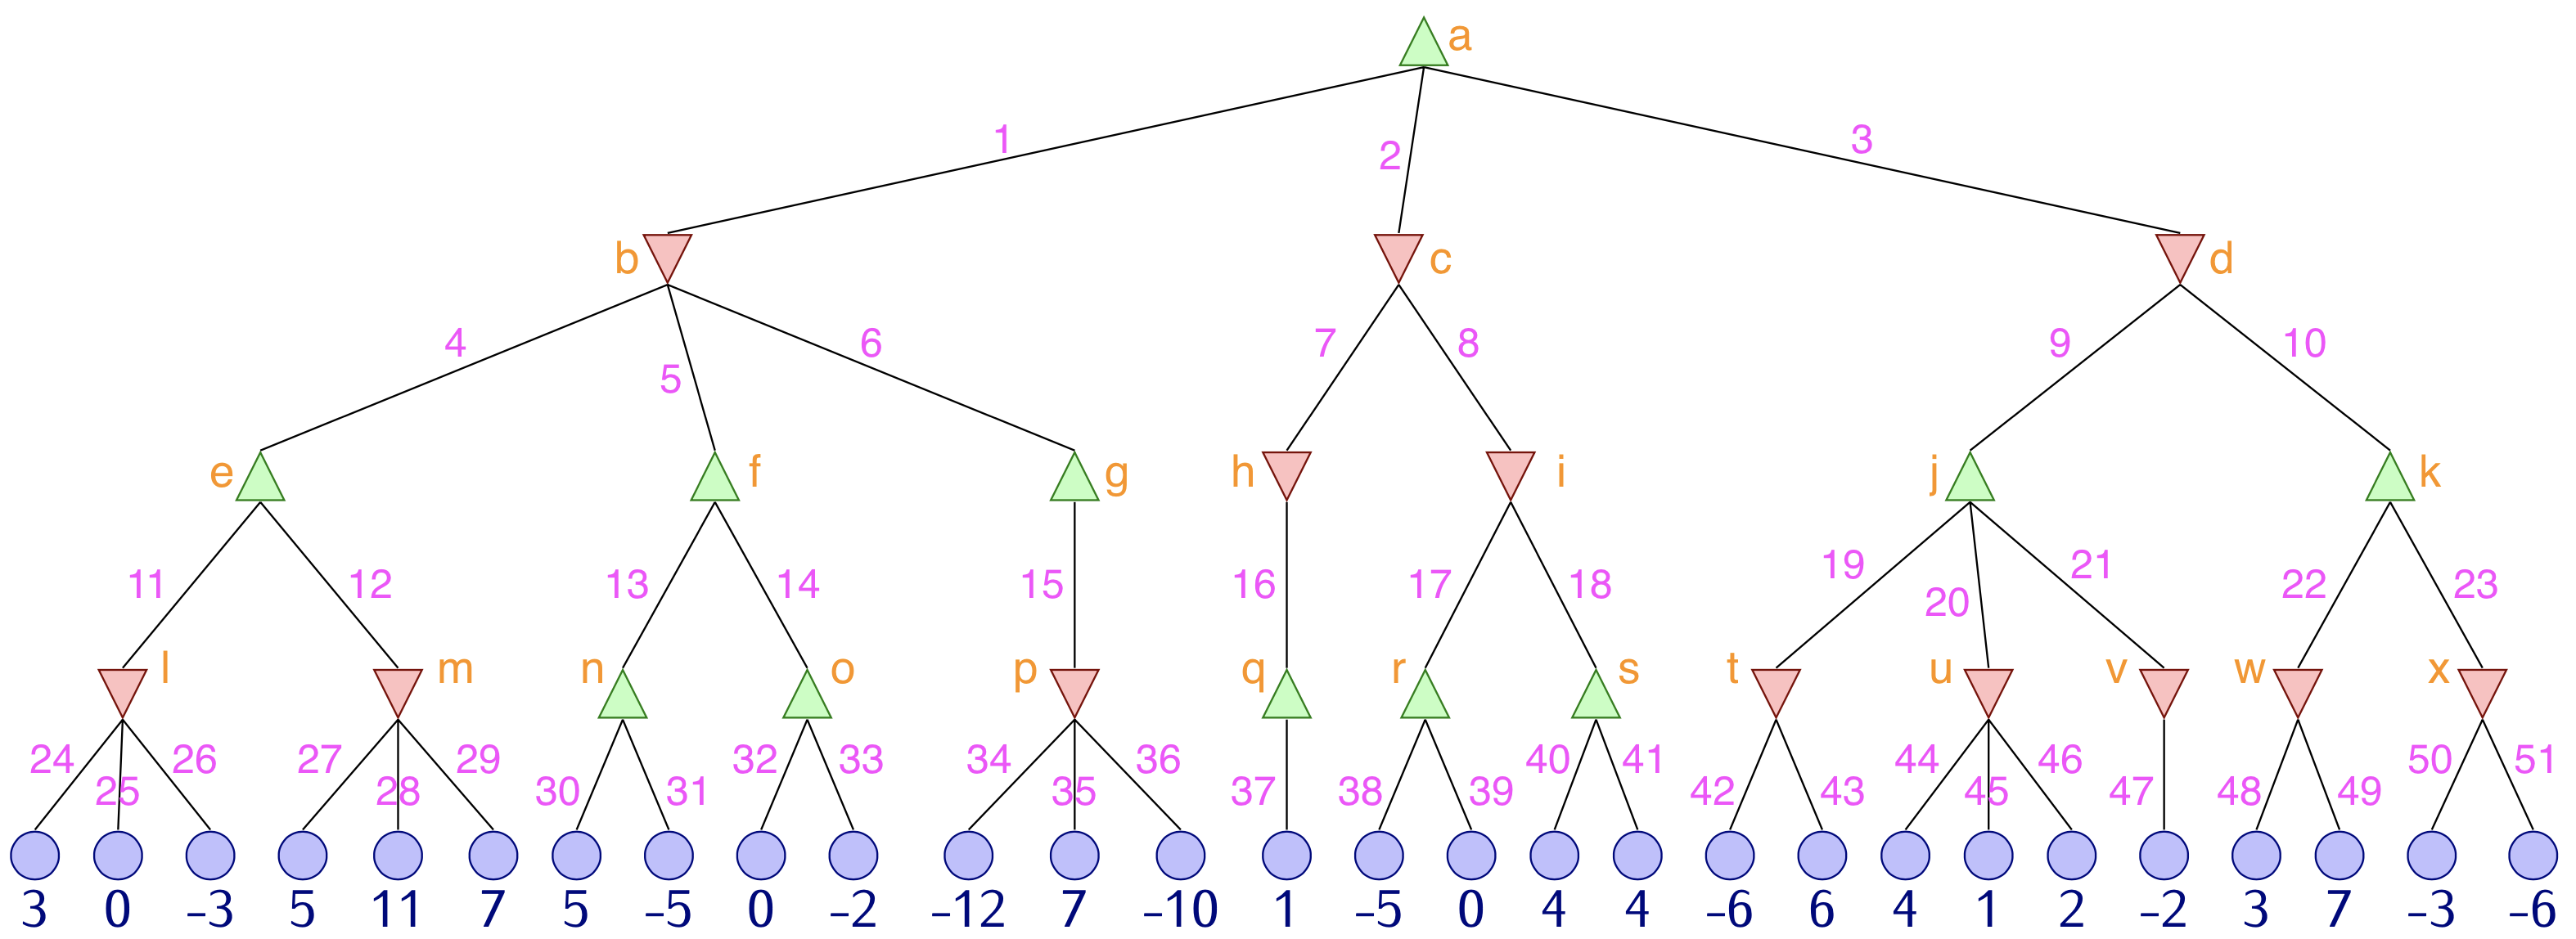
\includegraphics[width=\linewidth]{images/minimax_labelled.png}
\end{center}


\begin{enumerate}
\item Perform the MiniMax algorithm on the following tree, i.e.
      put a value to each node. What move should the root player do? \textbf{(1~pt)}
      
      \textit{Assign a numerical value to each node, and indicate the move (i.e.\! 1, 2, or 3) to perform:}
\end{enumerate}
      \begin{answers}[3cm]
      \begin{multicols}{5}
      \textbf{a: } %TODO Insert your answer here
      
      \textbf{b: } %TODO Insert your answer here
      
      \textbf{c: } %TODO etc.
      
      \textbf{d: }
      
      \textbf{e: }
      
      \textbf{f: }
      
      \textbf{g: }
      
      \textbf{h: }
      
      \textbf{i: }
      
      \textbf{j: }
      
      \textbf{k: }
      
      \textbf{l: }
      
      \textbf{m: }
      
      \textbf{n: }
      
      \textbf{o: }
      
      \textbf{p: }
      
      \textbf{q: }
      
      \textbf{r: }
      
      \textbf{s: }
      
      \textbf{t: }
      
      \textbf{u: }
      
      \textbf{v: }
      
      \textbf{w: }
      
      \textbf{x: }
      
      \textbf{Move: } %TODO Insert 1, 2 or 3 here
      \end{multicols}
	  \end{answers}



\begin{enumerate}
\item[2.] Perform the Alpha-Beta algorithm on the same tree.
      At each non terminal node, put the successive values of $\alpha$ and
      $\beta$. Cross out the arcs reaching non visited nodes. Assume a
      left-to-right node expansion. \textbf{(1~pt)}
      
      \textit{Indicate the successive $\alpha$ and $\beta$ values of each node in the table below. Separate successive values by a comma (,). Indicate at the bottom the identifiers of the branches that are cut (in increasing order, separated by a comma) (indicate only the branches where the cuts happen, i.e.\!} don't \textit{indicate the branches that are below a cut).}
\end{enumerate}

\begin{answers}[8cm]
      \begin{multicols}{2}
      \begin{tabular}{ccc}
      Node & $\alpha$ values & $\beta$ values\\
      \hline
      \textbf{a} &  &  \\ %TODO Insert your answer in the table (example: \textbf{a} & 1, 3, 2 & 5, 4 \\)
      \textbf{b} &  &  \\
      \textbf{c} &  &  \\
      \textbf{d} &  &  \\
      \textbf{e} &  &  \\
      \textbf{f} &  &  \\
      \textbf{g} &  &  \\
      \textbf{h} &  &  \\
      \textbf{i} &  &  \\
      \textbf{j} &  &  \\
      \textbf{k} &  &  \\
      \textbf{l} &  &  \\
      \textbf{m} &  &  \\ 
      \end{tabular}
      
      \begin{tabular}{ccc}
      Node & $\alpha$ values & $\beta$ values\\
      \hline
      \textbf{n} &  &  \\
      \textbf{o} &  &  \\
      \textbf{p} &  &  \\
      \textbf{q} &  &  \\
      \textbf{r} &  &  \\
      \textbf{s} &  &  \\
      \textbf{t} &  &  \\
      \textbf{u} &  &  \\
      \textbf{v} &  &  \\
      \textbf{w} &  &  \\
      \textbf{x} &  &  \\
       &  &  \\
      \end{tabular}
      \end{multicols}
      
\textbf{Cuts:} %TODO Insert your answer here (example: 2, 4, 6, 8, 10)
\end{answers}





\begin{enumerate}
\item[3.] Do the same, assuming a right-to-left node expansion instead.  \textbf{(1~pt)}
\end{enumerate}

\begin{answers}[8cm]
      \begin{multicols}{2}
      \begin{tabular}{ccc}
      Node & $\alpha$ values & $\beta$ values\\
      \hline
      \textbf{a} &  &  \\ %TODO Insert your answer in the table (example: \textbf{a} & 1, 3, 2 & 5, 4 \\)
      \textbf{b} &  &  \\
      \textbf{c} &  &  \\
      \textbf{d} &  &  \\
      \textbf{e} &  &  \\
      \textbf{f} &  &  \\
      \textbf{g} &  &  \\
      \textbf{h} &  &  \\
      \textbf{i} &  &  \\
      \textbf{j} &  &  \\
      \textbf{k} &  &  \\
      \textbf{l} &  &  \\
      \textbf{m} &  &  \\ 
      \end{tabular}
      
      \begin{tabular}{ccc}
      Node & $\alpha$ values & $\beta$ values\\
      \hline
      \textbf{n} &  &  \\
      \textbf{o} &  &  \\
      \textbf{p} &  &  \\
      \textbf{q} &  &  \\
      \textbf{r} &  &  \\
      \textbf{s} &  &  \\
      \textbf{t} &  &  \\
      \textbf{u} &  &  \\
      \textbf{v} &  &  \\
      \textbf{w} &  &  \\
      \textbf{x} &  &  \\
       &  &  \\
      \end{tabular}
      \end{multicols}
      
\textbf{Cuts:} %TODO Insert your answer here (example: 2, 4, 6, 8, 10)
\end{answers}




\clearpage
\begin{enumerate}
\item[4.] Is there a node ordering that can lead to a more optimal pruning of the tree
(in the sense where the algorithm prunes more branches than in the two other
considered cases)? If no, explain why. If yes, give a new node ordering and the
resulting new pruning.  \textbf{(1~pt)}
      
      \textit{Insert an image below containing the reordered tree, with successive $\alpha$/$\beta$ values indicated next to each node, and where the branches that are cut by the algorithm are crossed out. This may either be an edited version of \texttt{minimax\_empty.png} (using paint, gimp, etc.), a photograph of a drawing you made by hand, etc. In any case, the image must be \textbf{clear} in order to be graded.}
\end{enumerate}

\begin{answers}[8cm]
%TODO Insert the path to your image between the {}. 
% Possibly adjust the scale parameter so your image fits in the box.
%\includegraphics[scale=.3]{...}
\end{answers}




\begin{enumerate}
\item[5.] How does Alpha-Beta need to be modified for games with more than two players? \textbf{(1~pt)}
\end{enumerate}

\begin{answers}[9cm]
%TODO Insert your answer here
\end{answers}





\clearpage
\section{Shobu (35~pts)}
\medskip

\subsection{Alpha-Beta agent (4 points, to be submitted on Inginious)}
\medskip


\subsection{Monte-Carlo Tree Search agent (5 points, to be submitted on Inginious)}
\medskip


\subsection{Warm-up questions (3 points)}
\begin{enumerate}
\item[1.] What is the branching factor at the start of the game? What is the mean empirical branching factor? (The branching factor is considered here as the number of possible moves that a player can do from a given state). \textbf{(1 point)}
\end{enumerate}

\begin{answers}[5cm]
    % TODO put your answer here
\end{answers}



\begin{enumerate}
\item[2.] What would be one (of the many) drawbacks of the simple heuristic that is imposed for the basic alpha-beta agent above? \textbf{(1 point)}
\end{enumerate}

\begin{answers}[10cm]
    % TODO put your answer here
\end{answers}



\begin{enumerate}
\item[3.] Considering the Monte-Carlo Tree Search algorithm, what is the hypothesis supporting the use of random simulation to estimate the win rate? Is this hypothesis always valid? \textbf{(1 point)}
\end{enumerate}

\begin{answers}[15cm]
    % TODO put your answer here
\end{answers}


\newpage
\subsection{Description of your agent (8 points)}
Describe in the boxes below what you have implemented for your contest agent. You can also mention things that you tried and did not work but focus on what you have submitted in the end.

\begin{answers}[21cm]
    % TODO explain your agent here    
\end{answers}

\begin{answers}[23cm]
    % TODO continue your answer here
\end{answers}

\begin{answers}[23cm]
    % TODO continue your answer here
\end{answers}



\newpage
\subsection{Comparison of agents (5 points)}
Describe here the comparison of the different agents: random, Alpha-Beta, MCTS and your agent (and others if you want!). Remember that it should be a statistical comparison. Describe how you compare the agents. Draw some observations and conclusions based on the results you have obtained.

\begin{answers}[20cm]
    % TODO explain your comparison method and draw conclusions
\end{answers}

\begin{answers}[23cm]
    % TODO continue your answer here
\end{answers}

\begin{answers}[23cm]
    % TODO continue your answer here
\end{answers}


\subsection{Contest (10 points, to be submitted on Inginious)}



\end{document}
